\thispagestyle{plain}
\newpage
\section{Implementation}\label{sec:implementation}

\normalsize

\subsection{Start Small, Aim Big}\label{subsec:start-small-aim-big}

Section~\ref{sec:requirement-capture} details how the~\gls{mvp} for the project was formulated from the system requirements.
Given the complexity of the project,
it was advantageous to break down the elements of the system into smaller,
more atomic tasks that each worked towards a requirement.
Some of these discrete tasks can be seen in Figures~\ref{fig:timeline1},~\ref{fig:timeline2}, and ~\ref{fig:timeline1}.
By breaking down tasks in this way,
it was
easier to make incremental progress
rather than be overwhelmed by the complexity of the overall project.
The development strategy was to reach the~\gls{mvp}, overcome obstacles along the way,
and then refine further based on feedback from users.
Since much of the~\gls{mvp} was based on the system's functionality,
there was not a focus on the user experience at the outset of the project;
a flashy front-end was low on the initial list of priorities.

\subsection{Continuous Integration / Continuous Deployment}\label{subsec:continuous-integration-continuous-deployment}

As seen in Figure~\ref{fig:final_design}, the project is made up of a number of discrete modules that link together.
Furthermore, the~\gls{react} front-end comprises a number of interlinked components.
The development process saw the steady addition and refinement of modules and components to reach the final version.
However, given the interconnectedness of the system,
it was important to ensure that changes to the project did not affect older modules or components.
A common method of avoiding these breaking changes in industry is
to use~\gls{cicd}~\citep{duvall2007continuous, miller-ci}.

A~\gls{cicd} pipeline was set up using a combination of the Git version control software and~\gls{amplify}.
Each time a commit was pushed to the repository,
a build of the project was executed and then immediately deployed to an online environment.
As a part of the build,
a suite of~\gls{playwright}\footnote{In addition to end-to-end testing, an update to~\gls{playwright}'s feature set allowed for the testing of individual~\gls{react} components that could be mounted and tested independantly from one another.} automated tests was run
to ensure that the functionality previously established had not been compromised by the new commit.
Using this workflow, it was easy to identify issues when they occurred.

\begin{figure}[!htb]
    \minipage{\textwidth}
    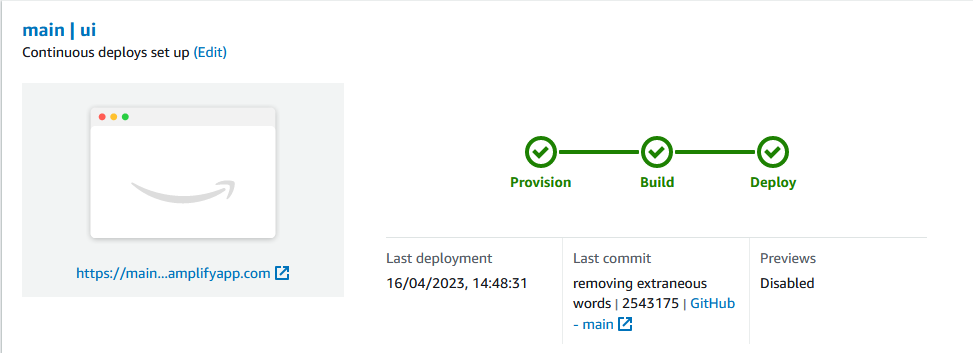
\includegraphics[width=\linewidth]{amplify}
    \caption{A screenshot of the~\gls{amplify} dashboard showing the successful provisioning, building, and deployment of a branch from the project repository}\label{fig:amplify}
    \endminipage
\end{figure}

This workflow enabled the use of parallel builds, which were utilised when the time came for user testing.
~\gls{amplify} is able to create a separate build and deployment for different branches of a GitHub repository
(Figure~\ref{fig:amplify}).
A version of the project was deployed for user testing alongside the main development branch.
This prevented new additions to the development branch disrupting the user testing version and deployment.

\subsection{Trials and Tribulations}\label{subsec:trials-and-tribulations}
During development of the project, a number of challenges and problems were encountered.
The project required the learning of a range of new pieces of software,
such as the~\gls{aws}~\gls{sdk} and~\gls{docker}.
This meant
that most delays to the project were due to insufficient knowledge
that needed to be corrected through reading documentation and examples that are hosted online.
However, some issues were far more significant and will be detailed below.

\subsubsection{The Recursion Incident}\label{subsubsec:recursion-incident}

The major incident of the project stemmed from the accidental over-allocation of~\gls{aws} resources.
A previous version of the orchestrating~\gls{aws-step-function} was triggered
when a file was uploaded to a~\gls{s3} bucket.
The~\gls{aws-step-function} then triggered the source-separation~\gls{aws-lambda} function
which contained a bug where the output of the function was deposited to the originating s3 bucket.
The depositing of the resultant stems then triggered another~\gls{aws-step-function} for each stem
deposited because of the aforementioned triggering rule.
Since the output of the source separation function was (at this point) two stems,
there was a recursive re-triggering of the step function
which increased the number of invocations and stored output stems at a quadratic rate.
Making matters worse,
this error was not noticed for at least a period of twenty minutes\footnote{As this author was on the London Underground!}.
This recursive invocation, despite triggering a number of Lambda throttles,
resulted in a large bill from~\gls{aws} since there is a charge per invocation (Figure~\ref{fig:incident-invocations}).
In addition,
the size of the files created was 1.3 TB,
and there were additional charges from~\gls{s3} due to the amount of data created and stored via~\gls{api} calls
(Figure~\ref{fig:incident-storage}).

\begin{figure}[!htb]
    \centering
    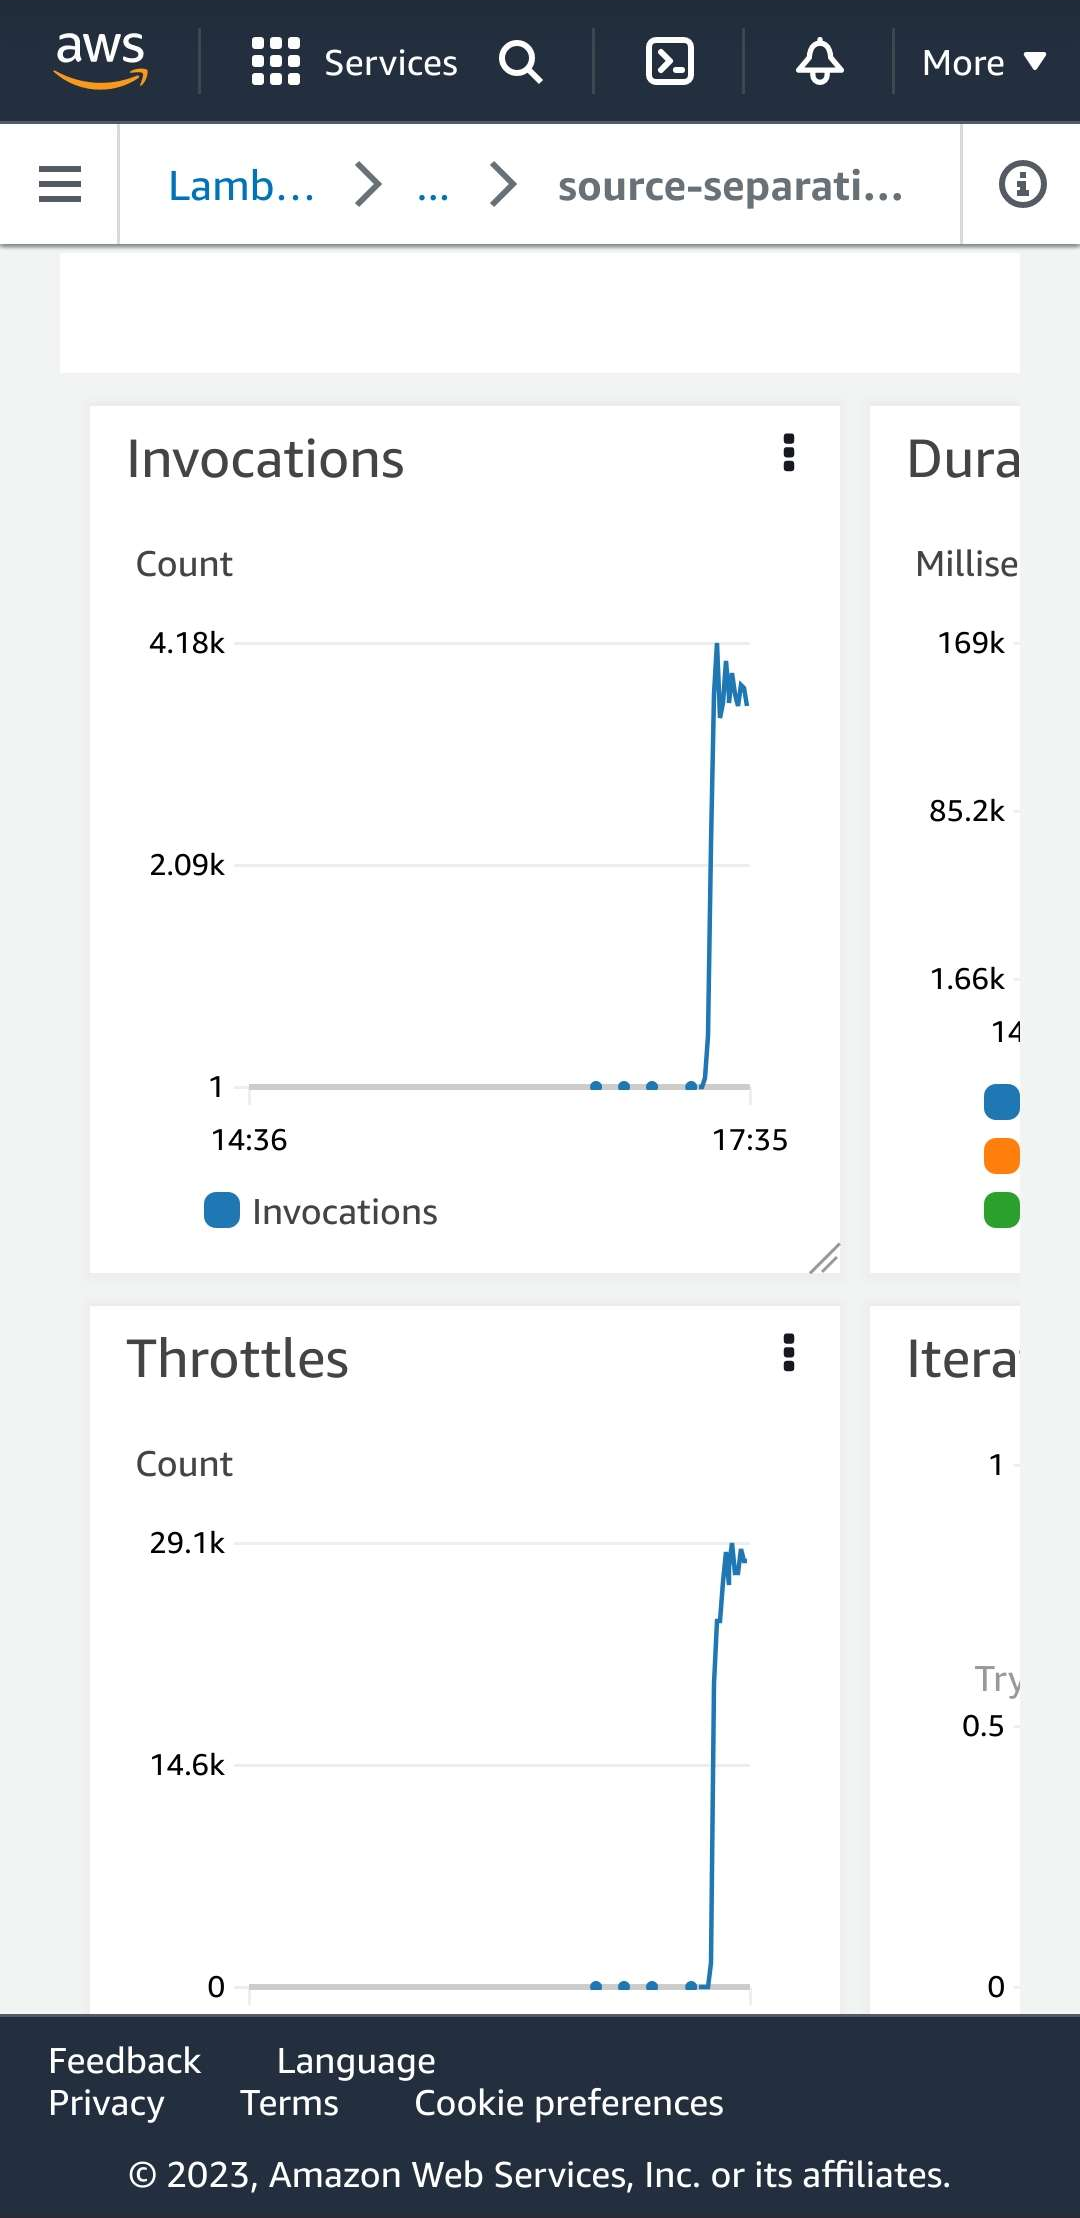
\includegraphics[height=20cm, keepaspectratio]{incident-invocations}
    \caption{A graph of the number of invocations and throttle over the time of the incident}\label{fig:incident-invocations}
\end{figure}

\begin{figure}[!htb]
    \centering
    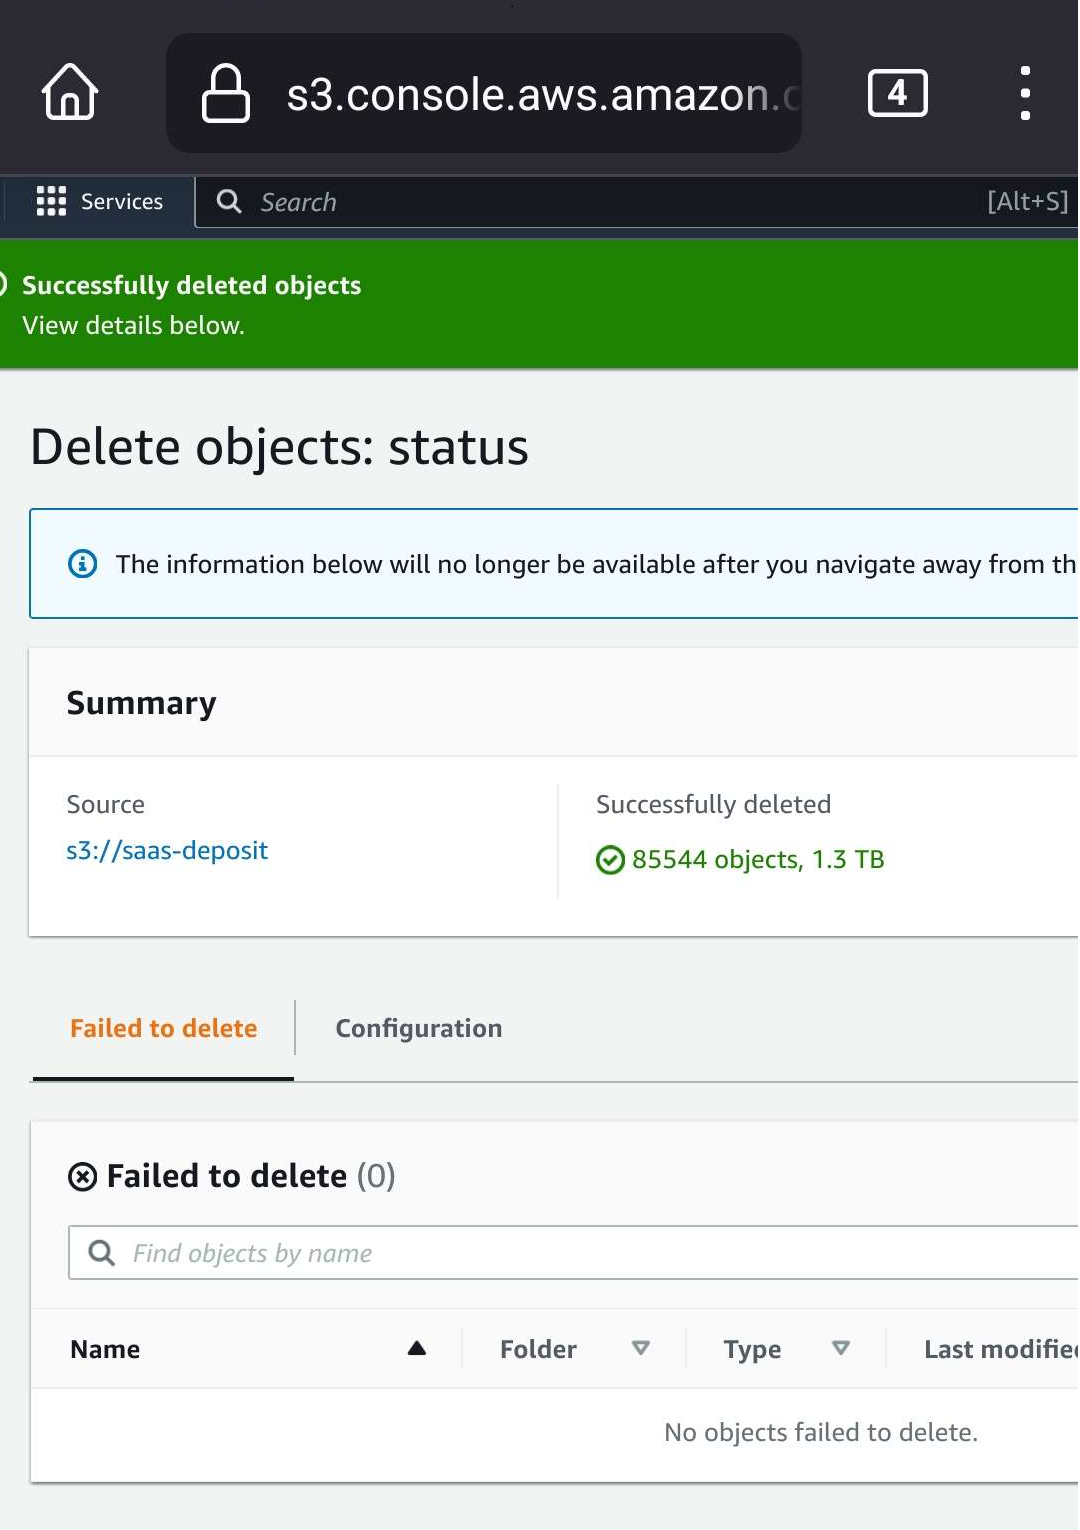
\includegraphics[height=20cm, keepaspectratio]{incident-storage}
    \caption{The size of the total objects deleted from the~\gls{s3}} bucket\label{fig:incident-storage}
\end{figure}

Thankfully~\gls{aws} customer service was understanding and forgave the charges
incurred on that day since it was a mistake.
However,
the situation stands as evidence
that developing for public cloud services poses a tangible risk as identified in~\ref{subsec:business-risks}.
The breakdown of the usage costs on the day of the incident can be found in Figures~\ref{fig:cost-graph} and~\ref{fig:cost-breakdown}.

\begin{figure}[!htb]
    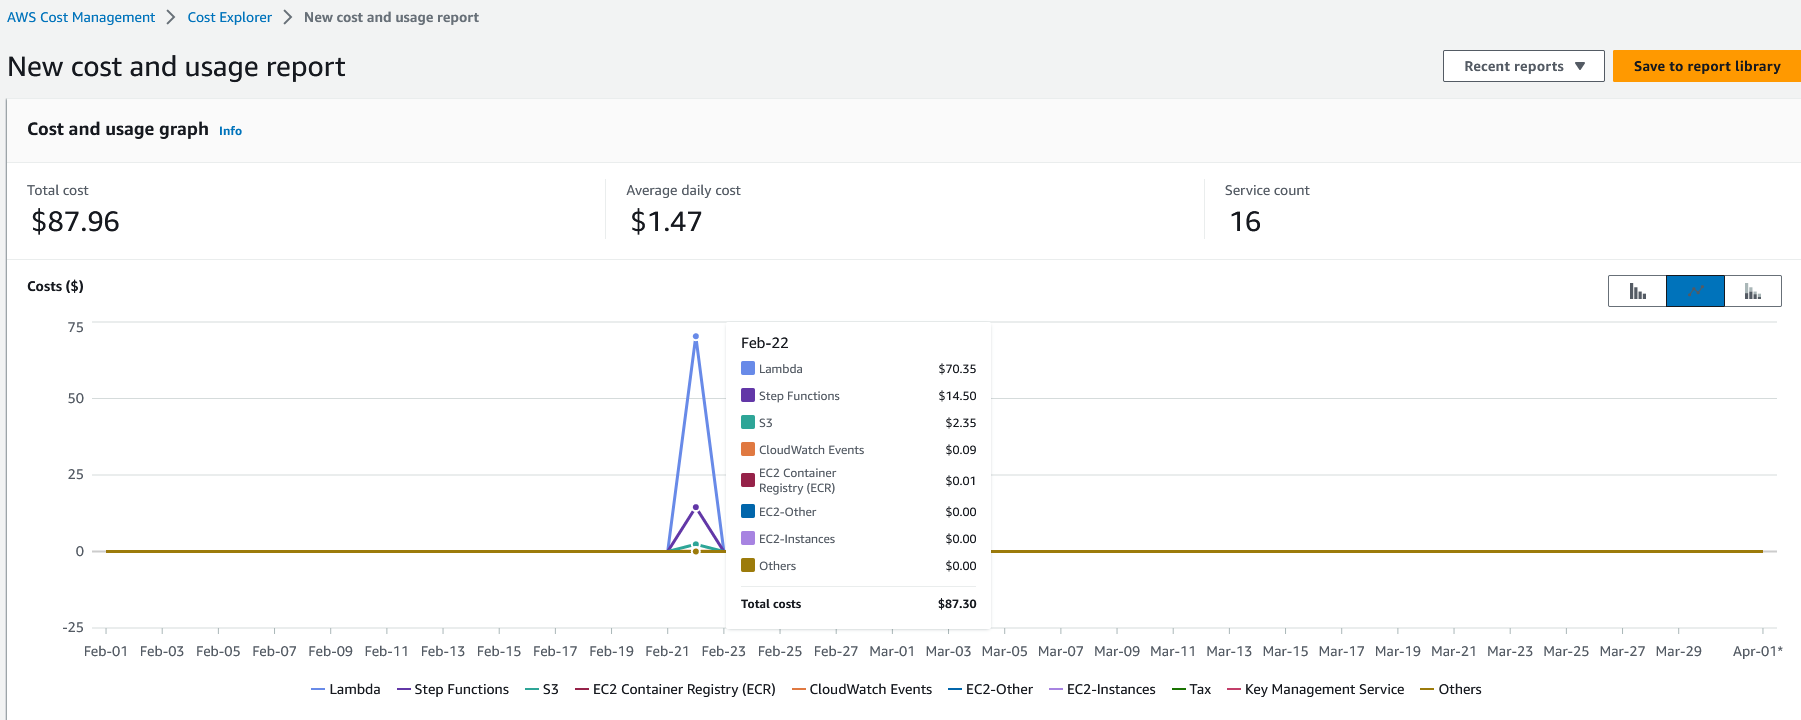
\includegraphics[width=\linewidth]{cost-graph}
    \caption{A graph showing the distribution of accidental charges in a wider billing period}\label{fig:cost-graph}
\end{figure}

\begin{figure}[!htb]
    \centering
    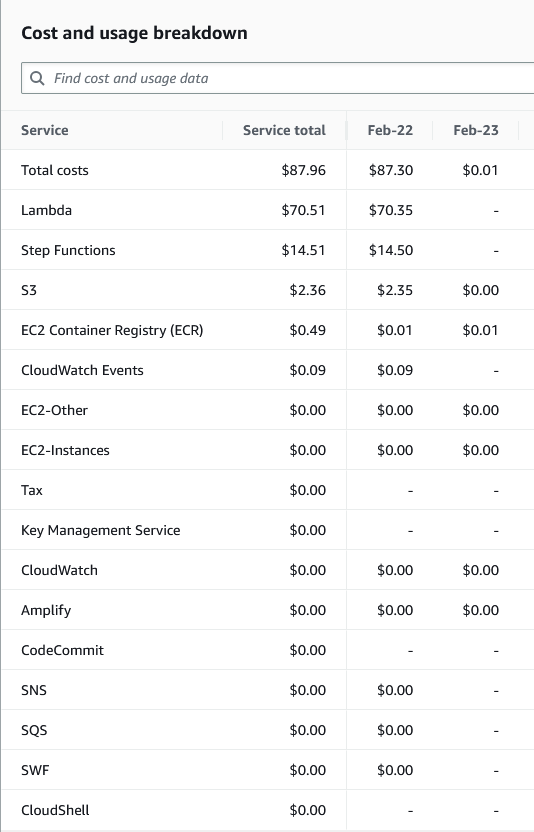
\includegraphics[height=20cm, keepaspectratio]{cost-breakdown}
    \caption{A granular breakdown of AWS costs on the day of the incident compared to the total costs for the duration of development. Fields with the value of \$0.00 mean that the service is in use, but hasn't used enough to incur charges}\label{fig:cost-breakdown}
\end{figure}

\subsubsection{Over-scoping}

One of the unexpected tests in the product's development was learning the importance of the user experience with customer-facing products.
As mentioned previously,
user testing revealed that while the functionality of the product was solid,
there was a lot of room for improvement in making the service effective at demonstrating the technology it uses.
The re-design of the front-end was significant
and required extra development time that put pressure on other areas of the project,
such as writing the report and creating the presentation video.
While the final product delivered the improvements requested from user testing,
there was too much work that existed out of the feasible scope of the project.

As a part of this work, a host of new technologies needed to be learnt in order to deliver the final product.
The amount of time needed for learning new technologies was not accounted for effectively in the planning stage.
For many of these technologies, there was little or no experience developing with them
and required significant time investment in order to use them effectively.
Had they not been included in the scope of the project, far less time would have been required.
